\meetingheader
    {Mar 17, 2026}
    {ae1fc12}
    {\meetinglinks{
        \meetinglink{Routine Framework}{https://arxiv.org/abs/2507.14447}
    }}
    {\begin{itemize}
        \item Previous single-agent policies (LLMPolicy, ModalPolicy) failed: wandering, hallucinated APIs, destructive curation spirals
        \item New RoutinePolicy architecture: Planner generates one phase at a time, Executor follows step-by-step with minimal context
        \item Three interaction modes: hypothesis (reasoning), exploration (data), implementation (transforms + research)
        \item Sub-agents (\texttt{coder}, \texttt{research}) ground decisions in evidence and validated code
    \end{itemize}}
    {}

%% ============================================================
%% SECTION 1: LIMITATIONS OF PREVIOUS IMPLEMENTATIONS
%% ============================================================

\section{Limitations of Previous Single-Agent Implementations}

Two single-agent policies were tested before the RoutinePolicy: LLMPolicy (free-form tool selection) and ModalPolicy (mode-switching with separate planning/execution phases). Across 11 runs spanning both architectures, no run achieved more than 49\% budget utilization, 3 of 11 never submitted a dataset, and 8 of 11 destroyed at least one dataset by removing 90\%+ of its rows.

\subsection{Research Does Not Transfer to Execution}

Agents produce correct research findings, then immediately contradict them during implementation.

In a ModalPolicy run, the agent concluded that ``VQAv2 answers are almost always short (1--3 tokens)'' and that word-count filters would be destructive. It then applied exactly those filters: \texttt{llava\_instruct} dropped from 157,710 to 54 rows (99.97\% removed), \texttt{vqav2} to 298 rows on the dataset it just said to protect, and \texttt{ocrvqa} to 86 rows.

This is not a capability problem. The knowledge exists but does not survive the boundary between reasoning and action.

\subsection{Errors Compound into Destructive Spirals}

Without a hypothesis-testing loop, failures escalate rather than self-correct.

In 10 of 11 runs, agents retried the same failing tool call with minor rephrasing rather than changing strategy (up to 12 consecutive identical attempts). When retries failed, agents escalated. One MAS agent switched from failed \texttt{coder} calls to \texttt{drop\_samples} and deleted every row from 3 of 5 datasets, rationalizing each as ``hostile rows.'' ModalPolicy runs averaged 5 rollbacks per episode, burning 30\%+ of steps on filter/rollback cycles without questioning the approach.

Table~\ref{tab:destructive} shows this pattern was universal across policies.

\begin{table}[H]
\centering
\small
\caption{Representative destructive filtering across policies. All runs used a 10,000-sample budget with 1,000-row dataset previews.}
\label{tab:destructive}
\begin{tabular}{llrrl}
\toprule
\textbf{Policy} & \textbf{Dataset} & \textbf{Before} & \textbf{After} & \textbf{Filter} \\
\midrule
MAS        & gqa, ocr\_vqa, coco & 1000 each & \textbf{0} each & \texttt{drop\_samples} (all rows) \\
Modal      & GQA                & 1000      & \textbf{3}       & reasoning-marker regex \\
Modal      & ocr\_vqa           & 1000      & \textbf{1}       & empty-field filter \\
Modal      & GQA                & 1000      & \textbf{1}       & answer-length threshold \\
LLM        & ocr\_vqa           & 1000      & \textbf{0}       & keyword filter ($\times$2) \\
\bottomrule
\end{tabular}
\end{table}

\subsection{Root Cause: No Hypothesis-Testing Loop}

All three architectures failed for the same reason: linear execution with no feedback. When a filter removed 99.97\% of data, the agent did not pause to ask why. It rolled back and tried softer thresholds, or escalated to deletion. Mode-switching added overhead without forcing genuine reflection.

Table~\ref{tab:aggregate} confirms the pattern is systematic across all policy types.

\begin{table}[H]
\centering
\small
\caption{Aggregate failure statistics across 11 single-agent runs (3~LLMPolicy, 4~ModalPolicy, 4~MAS). Budget: 10,000 samples.}
\label{tab:aggregate}
\begin{tabular}{lcccc}
\toprule
\textbf{Metric} & \textbf{LLM} & \textbf{Modal} & \textbf{MAS} & \textbf{Overall} \\
\midrule
Destructive filtering ($\geq$90\% removal) & 1/3 & 4/4 & 2/4 & 8/11 \\
Repeated identical failures ($\geq$5 retries) & 2/3 & 3/4 & 3/4 & 10/11 \\
Never submitted a dataset & 0/3 & 2/4 & 1/4 & 3/11 \\
Mean budget utilization & 42\% & 44\% & 50\% & 44\% \\
\bottomrule
\end{tabular}
\end{table}

%% ============================================================
%% SECTION 2: ROUTINE AGENTIC DESIGN
%% ============================================================

\newpage
\section{Routine Agentic Design}
\label{sec:routine}

The RoutinePolicy implements a planner-executor architecture inspired by the Routine framework~\cite{xuRoutineTaskDecompositionPlanning2025}. Rather than giving the LLM full control over a long conversation, the architecture separates \emph{ planning} from \emph{execution}.

\begin{figure}[H]
  \centering
  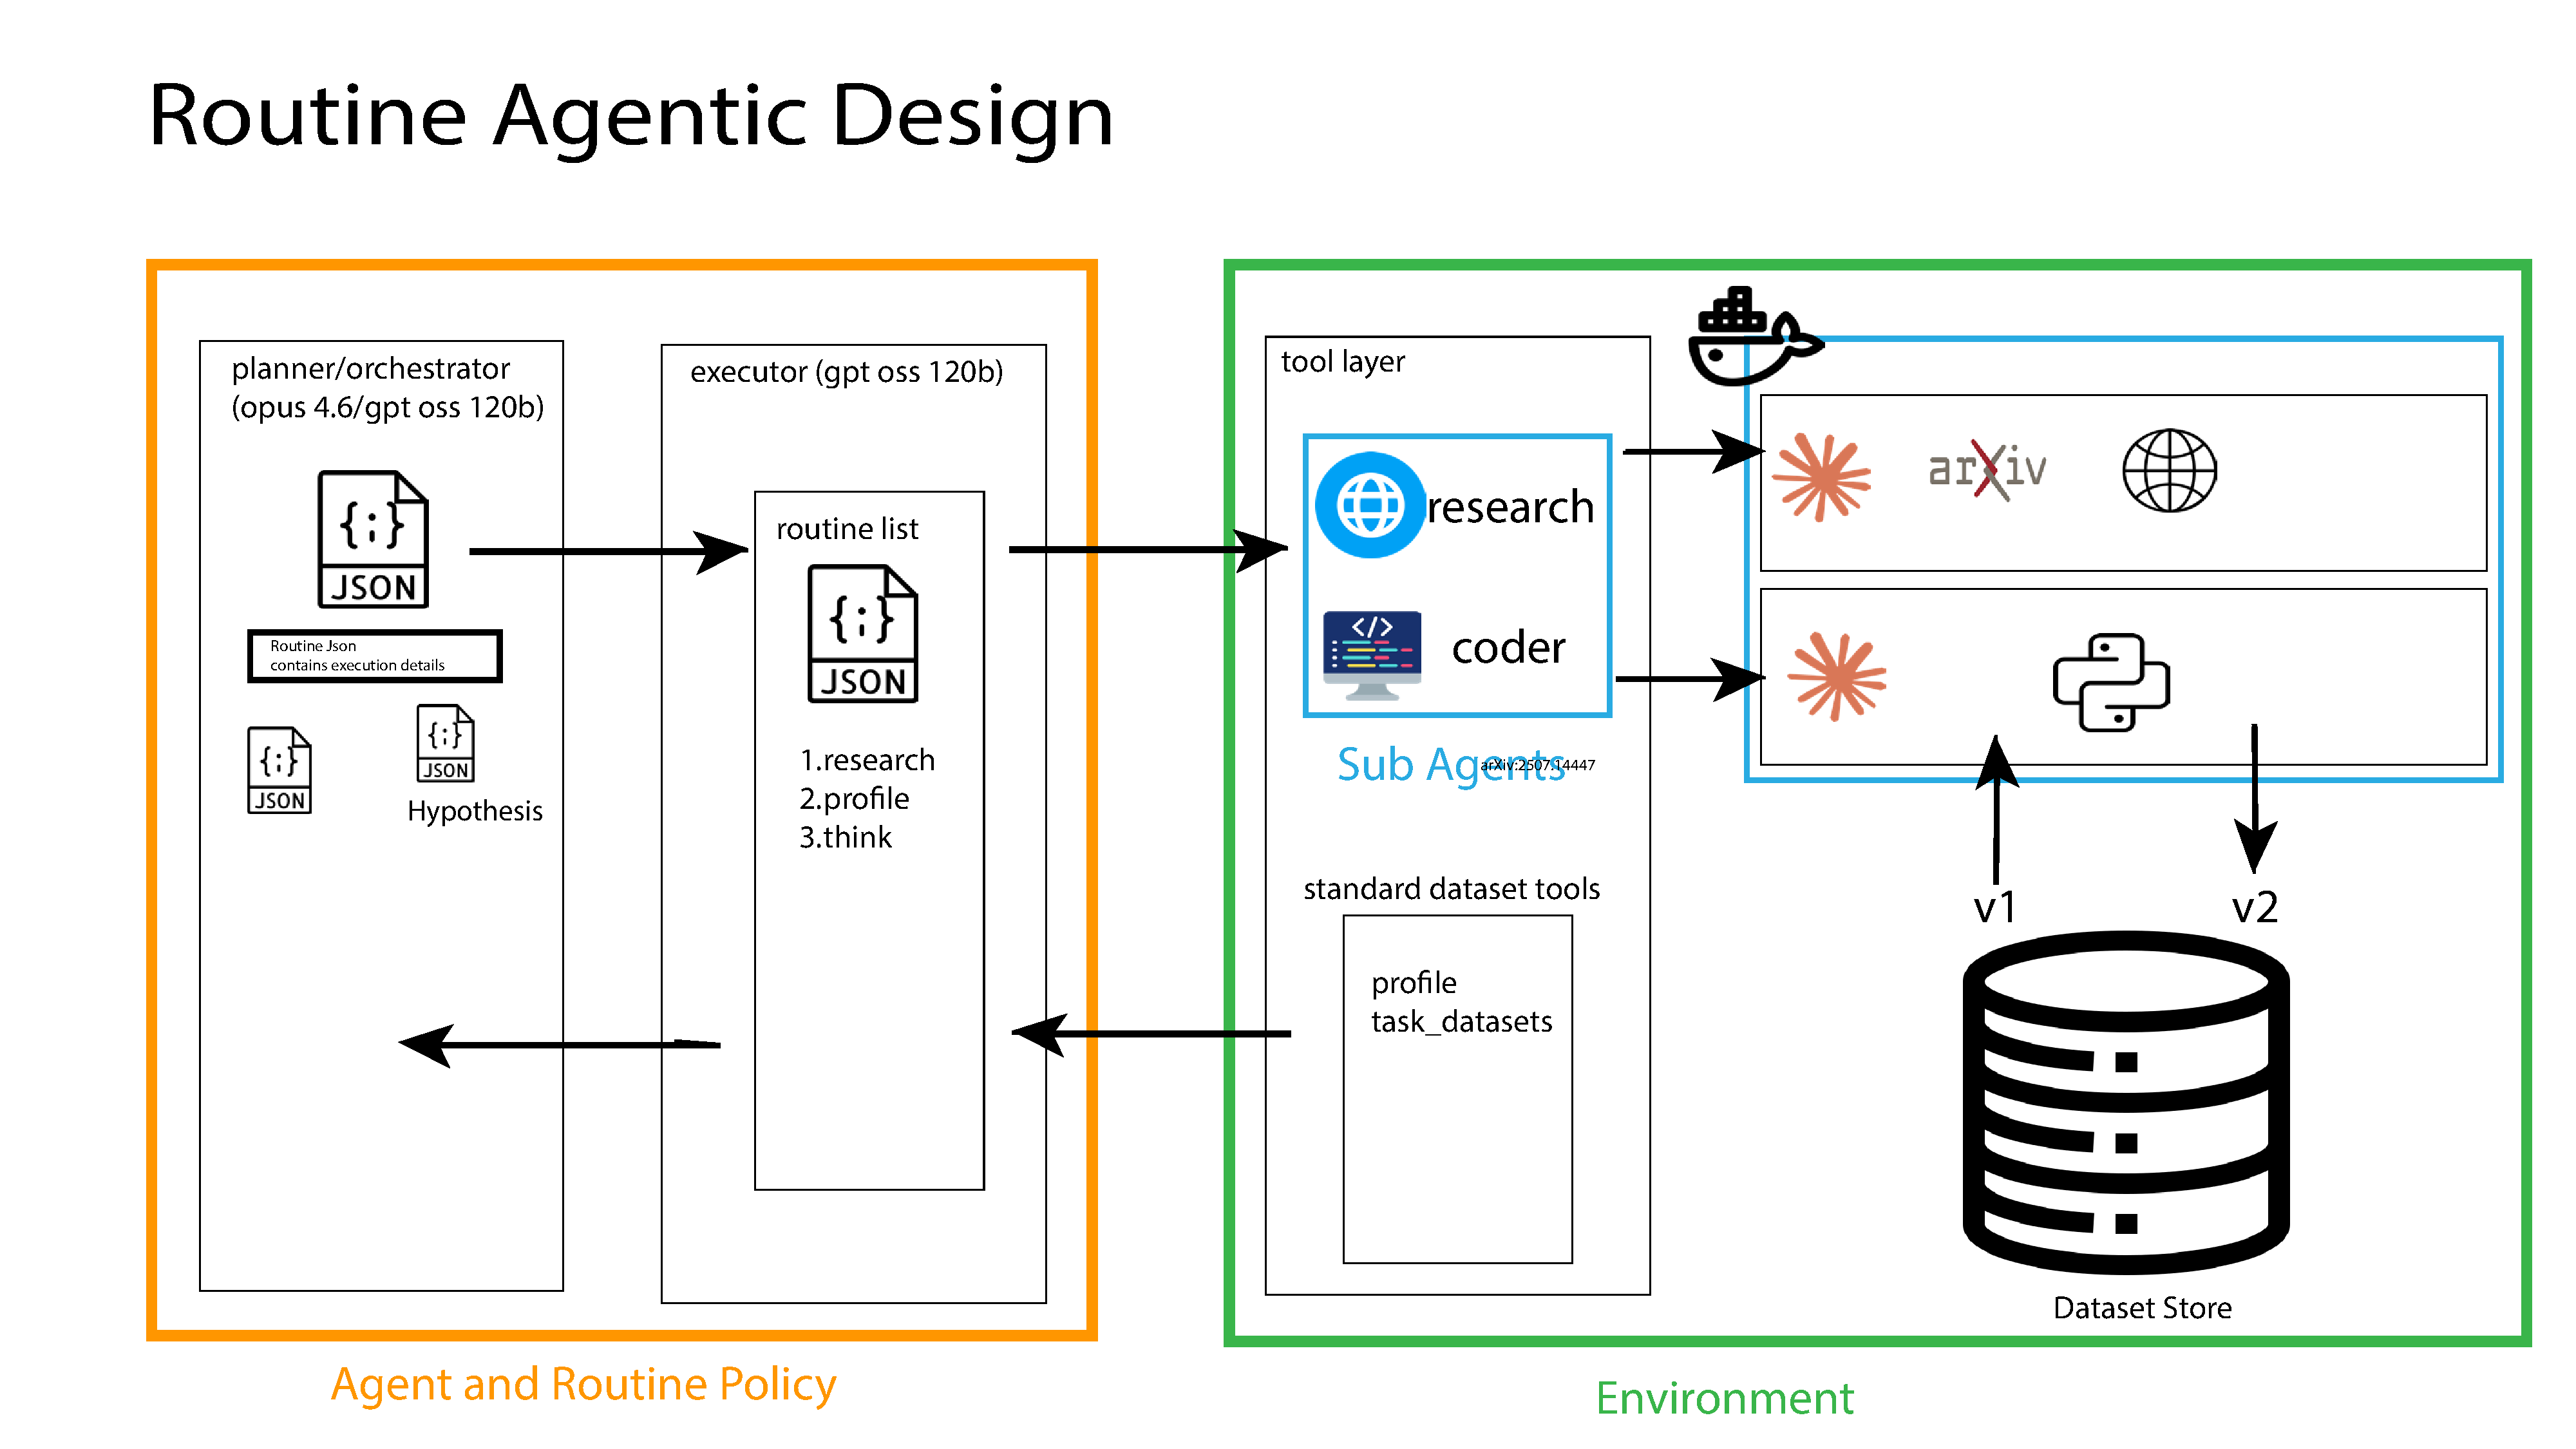
\includegraphics[width=0.95\linewidth]{routine_agent.pdf}
  \caption{Overview of the RoutinePolicy architecture...}
  \label{fig:routine-arch}
  \end{figure}

\subsection{Planner: One Phase at a Time}

The Planner (a Claude Code subprocess with full task context) generates \textbf{one phase at a time}, not a full upfront plan. Each phase is a linear sequence of 3--15 tool-call instructions. The Planner selects a phase type from three interaction modes:

\begin{itemize}
    \item \textbf{Hypothesis} --- internal reasoning and planning. The agent uses \texttt{think} to form or revise hypotheses, strategize, and plan budget allocation. No external tool calls needed; this is where the agent reasons about \emph{what to do next and why}.
    \item \textbf{Exploration} --- interaction with the data. Profile datasets, inspect samples, run analytical code (\texttt{execute\_code}) to understand distributions. The goal is to \emph{observe and confirm or reject hypotheses} before acting.
    \item \textbf{Implementation} --- interaction with the outside world and data transforms. Call \texttt{research} for domain knowledge, use \texttt{coder}/\texttt{execute\_code} to apply transforms, \texttt{rollback} to undo mistakes. This is where the agent \emph{acts on its understanding}.
\end{itemize}

\noindent A terminal \textbf{submission} variant includes \texttt{submit\_dataset} to end the episode.



\subsection{Example Run: 6 Phases, 33 Steps}

Table~\ref{tab:routine-phases} shows the phase structure from a representative curation-only run (FineVision5, 10K sample budget, no train/eval). The agent completed in 33 tool calls across 6 phases in 16 minutes.

\begin{table}[H]
\centering
\small
\caption{Phase trace from a RoutinePolicy curation run. Each phase is planned independently by the Planner based on prior phase results.}
\label{tab:routine-phases}
\begin{tabular}{clp{4cm}l}
\toprule
\textbf{Phase} & \textbf{Type} & \textbf{Tools} & \textbf{Steps} \\
\midrule
1 & hypothesis & think, task\_datasets, research, think & 4 \\
2 & exploration & execute\_code $\times$5, inspect\_samples $\times$3, think & 9 \\
3 & implementation & coder $\times$5, inspect\_samples $\times$2, execute\_code, think & 9 \\
4 & implementation & execute\_code $\times$5, think & 6 \\
5 & implementation & execute\_code, think & 2 \\
6 & implementation & execute\_code, think, submit\_dataset & 3 \\
\bottomrule
\end{tabular}
\end{table}

\paragraph{Research sub-agent (Phase 1, Step 3).}
The Planner's routine instructed: \emph{``Research what VLMEvalKit benchmarks measure and what training data characteristics improve scores.''} The \texttt{research} tool spawned a Claude Code subprocess with Brave Search and Semantic Scholar access. Key findings from the 6,860-character report:

\begin{itemize}
    \item \textbf{MMVet}: over-indexing on VQA short answers \emph{hurts} this benchmark; high-quality conversational data (LLaVA-Instruct) is the primary driver.
    \item \textbf{VQAv2}: 92.8\% of answers are single words---word-count filters would be destructive.
    \item \textbf{CoIDO}: 20\% data selection achieves 98.2\% of full-data LLaVA-1.5-7B performance.
    \item \textbf{Recommendation}: reduce VQA proportion to 20--30\% in favor of conversational data.
\end{itemize}

\paragraph{Coder sub-agent (Phase 3).}
The Executor described \emph{what} to do; the \texttt{coder} tool generated \emph{how}. Example for \texttt{vqav2}:

\begin{itemize}
    \item \textbf{Intent}: \emph{``Filter vqav2: remove rows where any turn has empty user or assistant. Deduplicate by first user question. Sample 2500 rows with seed=42.''}
    \item \textbf{Generated code} (1092 chars): validity filter $\to$ set-based dedup on first user turn $\to$ \texttt{np.random.default\_rng(42)} sampling $\to$ \texttt{result = pa.Table.from\_pylist(sampled)}
    \item \textbf{Result}: 82,772 $\to$ 2,500 rows (3\% retention via sampling, not destructive filtering)
\end{itemize}

\noindent Compare with ModalPolicy's approach to the same dataset: applied \texttt{MIN\_TURNS=3, MIN\_USER\_LEN=60} filters that reduced 82,772 $\to$ 298 rows (0.36\% retention), destroying the dataset.

\paragraph{Iterative error recovery (Phases 5--6).}
Phase 4 attempted to sample \texttt{ocrvqa} but the generated code imported \texttt{random} (blocked by the sandbox). Phase 5's Planner reasoning: \emph{``ocrvqa failed with ImportError---code likely used import random, which is blocked. Fix: no extra imports, just row indices with numpy.''} Phase 6 succeeded with a simpler approach.

